\chapter{Discussion}

This chapter reviews the development process of the Self-Controlled Aerial Navigation (SCAN) project. It describes how the plan-driven, waterfall methodology was applied, and discusses the main decisions made during each project phase. The chapter also covers challenges faced, reasons for key choices, and areas where the process could have been improved. In addition, it includes a risk analysis and suggestions for future work, providing guidance for teams who may continue developing the SCAN project.

\section{Methodology}

This section outlines the methodological approahc employed in the development of the Self-Controlled Aerial Navigation (SCAN) project. The methodology consists of project management techniques, version control strategies, an the utilization of various tools to ensure a structured development process.

\subsection{Project Management}
The project management approach for SCAN is centered around the use of GitHub Projects, an integrated tool within the GitHub platform. This tool provides different kinds of features to organise and keep track of project development.

\subsubsection{Kanban Board}
A Kanban board as shown in figure \ref{fig:kanban-board} is implemented using GitHub Projects to visualize and manage the workflow of tasks throughout the project lifecycle. 

The board is structured into five columns:

\begin{itemize}
    \item Roadmap: Contains high-level project milestones and objectives.
    \item Docs Todo: Lists documentation tasks that need to be completed.
    \item System Todo: Consists of pending system development tasks.
    \item In Progress: Shows tasks currently being worked on.
    \item Done: Contains completed tasks.
\end{itemize}

\FloatBarrier

\begin{figure}
    \centering
    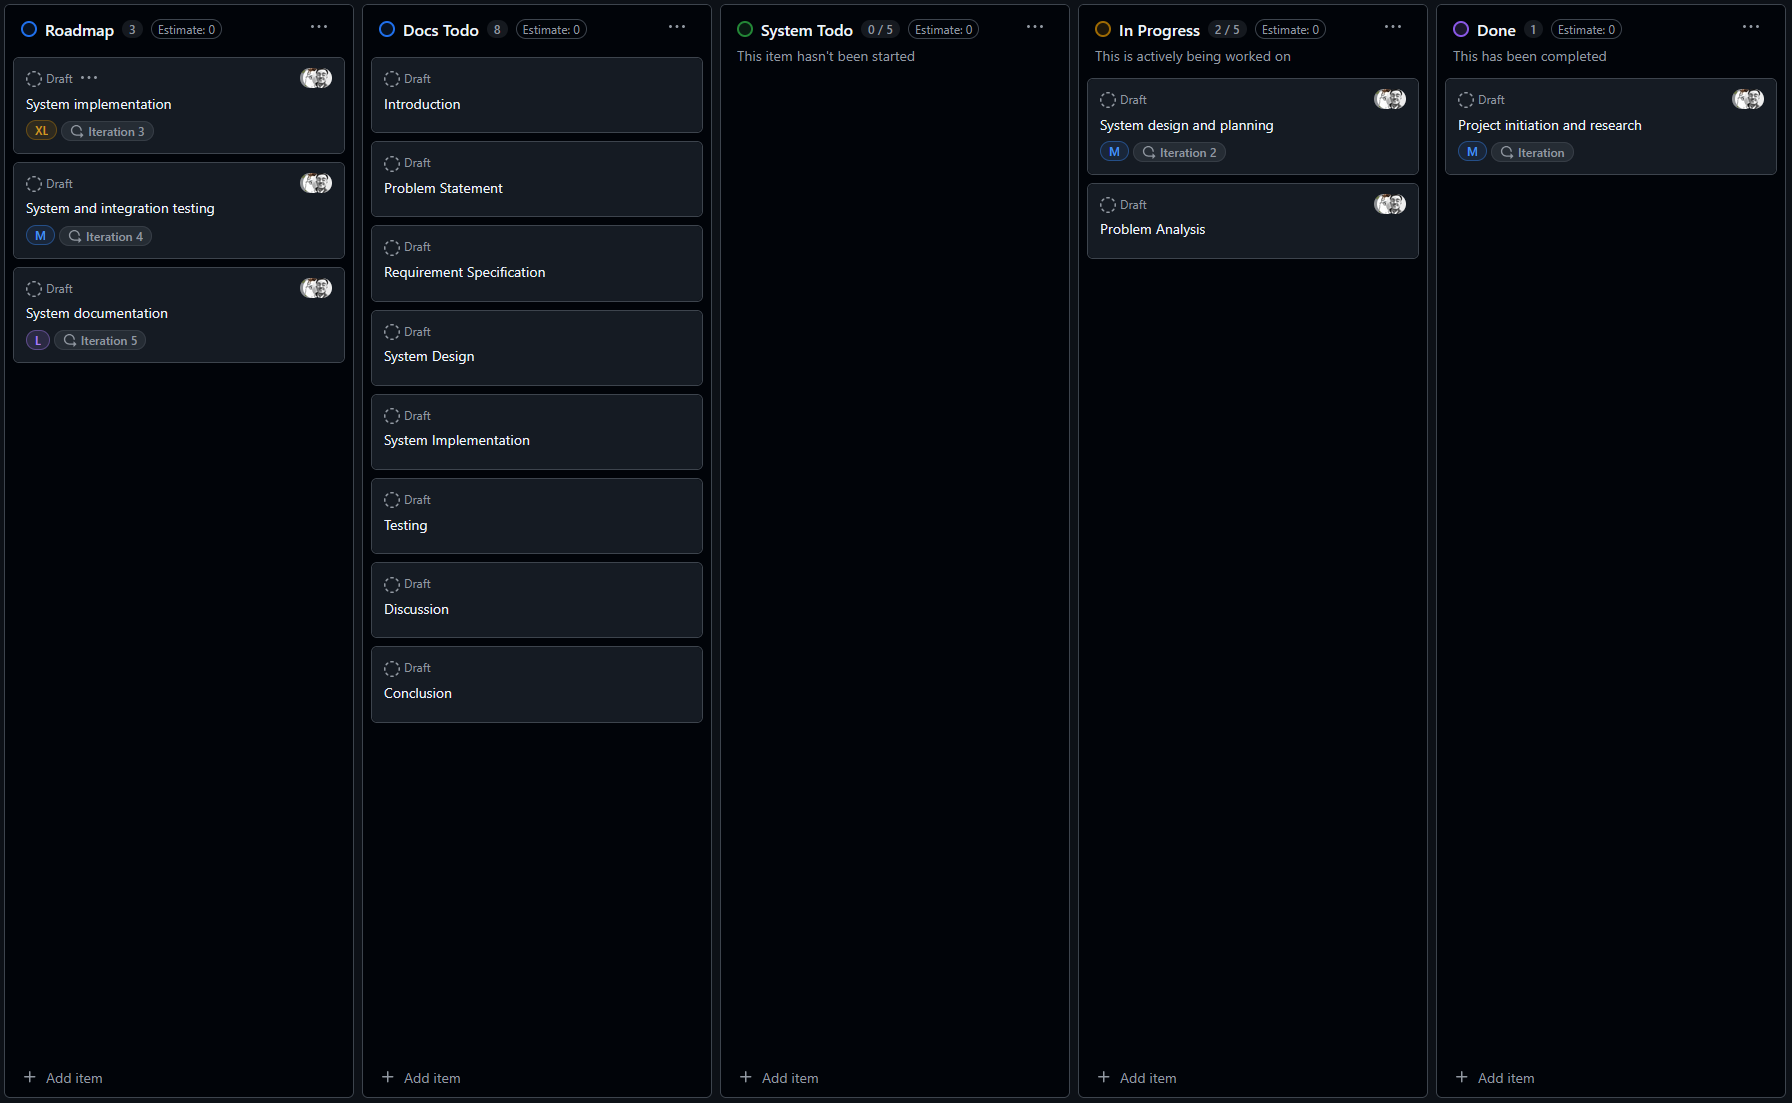
\includegraphics[width=1\linewidth]{7. Figures/Methodology/Kanbanboard.png}
    \caption{Kanban board utilized in the project}
    \label{fig:kanban-board}
\end{figure}

\subsubsection{Project Roadmap}

In addition to the Kanban board, a project roadmap is utilized to provide a timeline view of major project phases. The roadmap is divided into five phases:

\begin{enumerate}
    \item Project Initiation and Research (09/02/2025 - 21/02/2025).
    \item System Design and Planning (24/02/2025 - 07/03/2025).
    \item System Implementation (10/03/2025 - 02/05/2025).
    \item System and Integration Testing (05/05/2025 - 11/05/2025).
    \item System Documentation (12/05/2025 - 28/05/2025).
\end{enumerate}

Each phase is further broken down into specific tasks and objectives. For instance, the Project Initiation and Research phase includes:

\begin{itemize}
    \item Defining the initial project scope and objectives.
    \item Conducting literature review on drone navigation and control.
    \item Analyzing existing solutions and technologies.
    \item Drafting initial problem statement.
\end{itemize}

Similarly, the System Design and Planning phase consists of:

\begin{itemize}
    \item Refining problem statement and research questions.
    \item Developing the system architecture.
    \item Finalizing the report structure.
    \item Beginning initial report writing (problem analysis, statement, etc.).
\end{itemize}

This roadmap serves as a high-level guide for the project time, allowing for better resource allocation and also progress tracking. It should be noted however, that the project is not following the waterfall model but instead a more iterative model allowing for adjustments throughout the process and more flexibility. 

\subsection{Version Control}
Version control is an important aspect of the development process to ensure code integrity and provide collaboration among the team members. For the SCAN project, Git is employed as the version control system, with GitHub serving as the remote repository host.

\subsubsection{Branching Strategy}
A feature-based branching strategy is adopted for the project. The main branch serves as the stable, production-ready codebase, while the dev-main branch serves as the stage or development-level codebase. For each new feature or significant change, a new branch is created from the dev-main branch. After completion of a branch, it is merged into the dev-main branch and after finalizing a development stage, the dev-main development branch is merged into the main production branch.

The branching workflow is as follows:
\begin{enumerate}
    \item Create a new branch for a feature or bug fix from the dev-main branch.
    \item Develop and test the feature in isolation.
    \item Create a pull request for code review.
    \item After CI checks and approval, merge the feature branch back into the dev-main branch.
    \item Delete the feature branch after successful merge.
\end{enumerate}

\subsection{Continuous Integration (CI)}

While Continuous Integration (CI) is implemented in the SCAN project, Continuous Deployment (CD) is not deemed necessary due to the specific operational characteristics of the drone system. The reasons for this decision are as following.

\begin{enumerate}
    \item Local Execution Environment: The SCAN system is designed to operate with the backend running locally on a machine that directly interfaces with the drone or by uploading the final backend output directly into the drone for a disconnected autonomous operation. This local execution model differs significantly from typical web or cloud-based applications where CD is more commonly used.
    \item Autonomous Drone operation: The primary goal of the SCAN system is to enable autonomous drone navigation. Once the flight plan and navigation algorithms are loaded onto the drone, it is designed to operate independently without constant connection to an external system. As a fallback, the only connection to the drone would be between the backend and the drone itself, which would require the backend to be within range of the drone.
\end{enumerate}

GitHub Actions is utilized to set up CI workflows. These workflows are triggered on every push to the repository and on the creation of pull requests. The CI process includes the following steps:

\begin{enumerate}
    \item Code compilation: Ensures that the code builds successfully.
    \item Unit testing: Runs the project's unit tests to verify individual components.
    \item Integration testing: Performs tests on integrated components to verify behavior of multiple integrated components.
\end{enumerate}

If any of these steps fail, the CI process is halted, and the team members are notified of the failure. 

\subsection{Communication and Collaboration}
Communication and collaboration are very important for the success of the SCAN project. The following practices are implemented to ensure this:

\begin{itemize}
    \item Team meetings: Project development 4 times a week (mostly) with informal meetings of project progress and upcoming tasks.
    \item Discord: Used for real-time communication and quick discussions.
    \item GitHub discussions: Issue descriptions and comments are perhaps going to be utilized for longer, asynchronous conversations about project direction and technical decisions.
    \item Shared documentation: Notion with a project-focused directory for project-relevant information.
\end{itemize}

\section{What could we have done different?}

\subsection{Potential Improvements Through Early Risk Analysis}

A structured risk analysis at the start of the project could have prevented several avoidable issues. One of the main problems was the immediate reliance on the actual drone for testing. The project had access to a simulation tool designed for safe and controlled testing of navigation and control algorithms. However, the simulation tool was not set up or used until after the drone had already been damaged during early physical tests.

If the simulation tool had been configured and integrated into the workflow from the beginning, initial development and testing could have taken place in a virtual environment. This would have reduced the risk of hardware damage and allowed for faster iterations without the delays caused by repairing or replacing physical equipment. The lack of early simulation testing resulted in unnecessary downtime when the only available drone was damaged, which could have been avoided.

An early risk analysis would likely have identified the risks associated with hardware dependency and highlighted the benefits of simulation-based testing. This approach would have allowed the team to validate core functionalities and catch errors in a safe environment before moving to real-world tests. For future projects, setting up and prioritizing the use of simulation tools at the start is recommended, as it minimizes the risk of equipment failure and project delays.

\section{Future Work}

\subsection{The Advantages of Thermal Cameras for Drone-Based Water Rescue}

The current drone-based water rescue solution utilizes standard RGB cameras and a YOLOv8 model to detect humans in open water. While effective during daylight and clear weather, this approach has reliability limitations in challenging conditions. Integrating thermal cameras would address these limitations and improve performance.

\subsubsection{Enhanced Reliability with Thermal Imaging}

Thermal cameras detect heat signatures rather than visible light, offering key advantages:

\begin{itemize}
    \item \textbf{Operation in Low-Light and Night Conditions:} Standard cameras fail after sunset, while thermal cameras enable 24/7 operation\cite{advexure_thermal_sar}.
    \item \textbf{Performance in Adverse Weather:} Thermal imaging penetrates fog and ignores water surface glare, maintaining detection capability during rain or poor visibility.
    \item \textbf{Faster Detection:} Heat signatures simplify human identification for AI models, reducing missed detections from camouflage or shadows.
\end{itemize}

\subsubsection{Combining Camera Technologies for Optimal Results}

For the most effective search and rescue operations, especially in varied lighting and weather conditions, combining multiple camera types is recommended:

\begin{itemize}
    \item \textbf{Daytime Operations:} Using both RGB cameras and thermal cameras allows for cross-verification, improving detection accuracy. RGB cameras provide high-resolution visual information, while thermal cameras highlight heat signatures that might be missed in cluttered visual backgrounds.
    \item \textbf{Nighttime Operations:} A combination of thermal cameras and night vision cameras is ideal. Thermal cameras detect heat signatures in complete darkness, while night vision cameras amplify available light, providing additional visual context and helping to identify objects or obstacles that may not emit heat.
\end{itemize}

This multi-sensor approach increases the chances of detecting persons in the water under all conditions and reduces the likelihood of false negatives.

\subsubsection{Limitations and Cost Considerations}

\begin{itemize}
    \item \textbf{High Equipment Costs:} Thermal drones range from \$6,500 to \$24,000+ versus standard camera drones\cite{dslrpros_sar_drones}.
    \item \textbf{Environmental Constraints:} Reduced effectiveness when body and water temperatures are similar (e.g., after prolonged cold immersion). Thermal cameras cannot see through water, limiting detection if a person is submerged\cite{fireapparatus_thermal_water_rescue}. Combining thermal cameras with RGB or night vision cameras can help mitigate these limitations by providing additional visual information when thermal contrast is low or when a person is partially submerged.
    \item \textbf{Regulatory Challenges:} Additional restrictions may apply for nighttime or over-water operations.
\end{itemize}

\subsubsection{Comparative Summary}

\begin{table}[h]
\centering
\begin{tabular}{|l|l|l|l|}
\hline
\textbf{Feature} & \textbf{RGB Camera} & \textbf{Night Vision} & \textbf{Thermal Camera} \\ \hline
Daytime Operation & Yes & No & Yes \\ \hline
Nighttime Operation & No & Yes & Yes \\ \hline
Fog/Glare Performance & Limited & Limited & Excellent \\ \hline
Detection Reliability & Moderate & Moderate & High \\ \hline
Cost & Lower & Moderate & Higher \\ \hline
\end{tabular}
\caption{Comparison of camera systems for water rescue drones}
\end{table}

\subsubsection{Conclusion}

Thermal cameras substantially improve reliability for water rescue drones by enabling 24/7 operation and performance in adverse weather. Combining thermal imaging with RGB cameras during the day, and with night vision cameras during the night, provides the most robust solution for detecting persons in the water. While cost and regulatory factors require consideration, the life-saving potential and improved consistency make a multi-sensor approach the preferred choice for critical search and rescue missions.




\subsection{Multi-Drone Support}

While multi-drone functionality was not fully implemented in the current project iteration, preliminary exploration demonstrated its potential to significantly improve mission efficiency. A custom Python script was developed to simulate multi-drone operation by dividing search areas into segments, with each drone assigned a specific zone using proximity-based allocation. This section outlines the technical foundations and benefits observed during simulation.

\textbf{Key Technical Advantages}
\begin{enumerate}
    \item \textbf{Parallel Coverage:}
    \begin{itemize}
        \item Single-drone systems require sequential scanning of entire search grids.
        \item Multi-drone implementations split grids into non-overlapping segments (see Figure\ref{fig:multi_drone}), enabling simultaneous coverage.
        \item Simulation results showed a near-linear reduction in mission duration with each added drone (e.g., 2 drones $\approx$ 50\% time reduction).
    \end{itemize}
    \item \textbf{Proximity-Based Assignment:}
    \begin{itemize}
        \item Drones are assigned grid segments closest to their predefined start points.
        \item This minimizes initial travel distance compared to centralized allocation methods.
    \end{itemize}
    \item \textbf{Collision Avoidance:}
    \begin{itemize}
        \item Exclusive grid assignments eliminate mid-air collision risks during missions.
    \end{itemize}
    \item \textbf{Scalable Architecture:}
    \begin{itemize}
        \item The core path planning algorithm remained unchanged in simulations.
        \item New drones only require segment assignment logic and start point coordinates.
    \end{itemize}
\end{enumerate}

\textbf{Search \& Rescue Implications}

For aquatic person detection scenarios, multi-drone deployment could:
\begin{itemize}
    \item Reduce critical response times in time-sensitive emergencies
    \item Enable coverage of larger search areas without sacrificing resolution
    \item Provide redundancy if individual drones malfunction
\end{itemize}

\textbf{Implementation Challenges}

The simulation revealed two key requirements for practical implementation:
\begin{enumerate}
    \item \textbf{Centralized Coordination:} A master system to allocate grid segments and monitor drone statuses.
    \item \textbf{Hardware Standardization:} Identical drone specs for consistent flight performance and camera capabilities.
\end{enumerate}

While full integration remains future work, the simulation (see Figure\ref{fig:multi_drone}) validated the core technical approach. Implementing multi-drone support would require additional development in fleet coordination interfaces and real-time status monitoring, but the foundational path planning architecture appears directly adaptable.

\begin{figure}[h]
    \centering
    \includegraphics[width=0.8\textwidth]{multi_drone_simulation}
    \caption{Simulation output showing three drones covering partitioned grid segments using proximity-based assignment}
    \label{fig:multi_drone}
\end{figure}
